\chapter{Конструкторский раздел}
\label{cha:design}

\section{IDEF0}

На рисунке \ref{fig:idef0} приведена диаграмма состояний IDEF0 нулевого уровня, а на рисунке \ref{fig:idef1} --- диаграмма состояний IDEF0 первого уровня.

\begin{figure}[ph!]
	\center{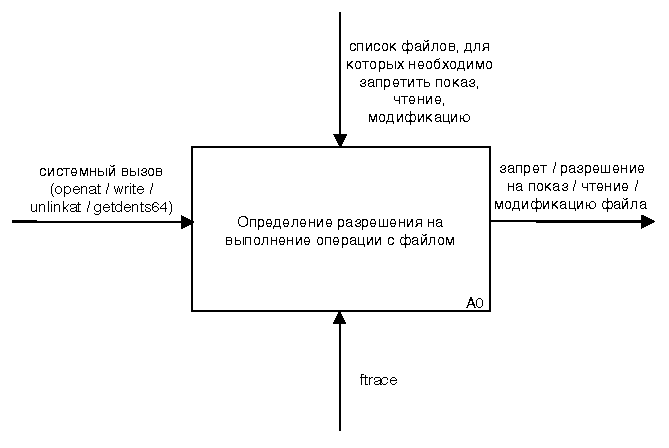
\includegraphics[scale=1.3]{img/idef0_0.pdf}}
	\caption{Диаграмма состояний IDEF0 нулевого уровня}
	\label{fig:idef0}
\end{figure}

\begin{figure}[ph!]
	\center{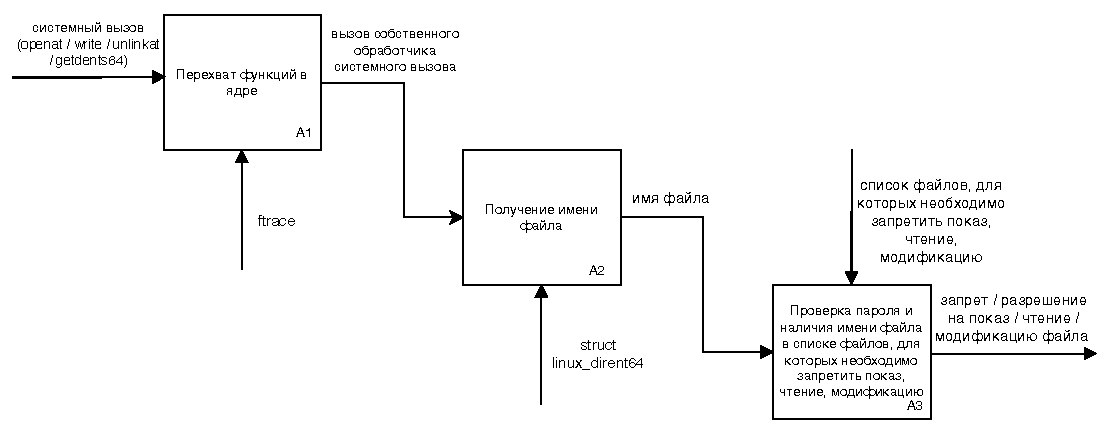
\includegraphics[scale=0.8]{img/idef0_1.pdf}}
	\caption{Диаграмма состояний IDEF0 первого уровня}
	\label{fig:idef1}
\end{figure}

\clearpage

\section{Алгоритм инициализации модуля}

\section{Алгоритмы функций--оберток}

\section{Структура программного обеспечения}

На рисунке \ref{fig:struct} представлена структура программного обеспечения.

\begin{figure}[ph!]
	\center{\includegraphics[scale=0.2]{img/start.png}}
	\caption{Структура программного обеспечения}
	\label{fig:struct}
\end{figure}

\section*{Вывод}
В данном разделе были рассмотрены алгоритмы работы сервера и обработки запроса.


